\documentclass{beamer}
% \usepackage{beamerthemesplit}
\usetheme{Madrid}
% \usepackage{pstricks}
\usepackage{graphicx}
\usepackage{mdwlist}
\usepackage{lineno, hyperref}
\usepackage{stackrel}
\usepackage{changepage}

\usepackage{amssymb,latexsym,amsmath,amsthm,bbm}
\usepackage{hyperref}
\usepackage{tikz}
\usepackage[english]{babel}
\usepackage[latin1]{inputenc}
\usepackage{multirow}
\usepackage{verbatim}
\usepackage{alltt}
\usepackage{mycommands}

% \usepackage{cmbright}
\renewcommand*\familydefault{\sfdefault}
\usepackage[T1]{fontenc}


\definecolor{wp-red}{RGB}{204,0,0}
\definecolor{wp-gray}{RGB}{51,51,51}
\definecolor{reynolds-red}{RGB}{153,0,0}
\definecolor{pyroman-flame}{RGB}{209,81,34}
\definecolor{hunt-yellow}{RGB}{253,215,38}
\definecolor{genomic-green}{RGB}{125,140,31}
\definecolor{innovation-blue}{RGB}{66,126,147}
\definecolor{bio-indigo}{RGB}{65,86,161}

\setbeamercolor{structure}{fg=wp-red}
\setbeamercolor{title}{bg=white, fg=wp-red}  % changes color on title page
\setbeamerfont{title}{series=\bfseries, size=\huge}
\setbeamerfont{author}{series=\bfseries, size=\large}
\setbeamerfont{institute}{series=\mdseries, size=\large}

\setbeamercolor{frametitle}{bg=wp-red, fg=white}  % changes color at top of frame
\setbeamerfont{frametitle}{series=\bfseries}
\setbeamercolor{title in head/foot}{fg=white, bg=wp-red}  % changes color for title in footer
\setbeamerfont{title in head/foot}{series=\bfseries}
\setbeamercolor{author in head/foot}{fg=white,bg=wp-gray}  % changes color for author in footer
\setbeamerfont{author in head/foot}{series=\bfseries}


\title[Rare Spatial Binary Regression] % (optional, use only with long paper titles)
{
  Rare Spatial Binary Regression
}
\author[S. Morris and B. Reich]{Samuel Morris (NC State)\\
        Brian Reich (NC State)}
\institute[NCSU]{}
\date{JSM 2015, Seattle}

\begin{document}

\begin{frame}\frametitle{\ }
\begin{center}
	\maketitle
\end{center}
\end{frame}

\begin{frame}{Motivation}
\begin{itemize} \setlength{\itemsep}{1em}
  \item Modeling and predicting rare occurrences in a spatial setting
  \begin{itemize} \setlength{\itemsep}{0.5em}
    \item \alert{Rare}: to mean not occurring often (e.g. 5\% or less)
    \item Based on binary regression, but incorporating methods for spatial extremes
  \end{itemize}
  \item Application: Species mapping (eBirds)
  \begin{itemize} \setlength{\itemsep}{0.5em}
    \item Cornell Lab of Ornithology and National Audubon Society
    \item In 2002, almost 50,000 bird sightings (starting year)
    \item March 2012, more than 3.1 million observations
    \item Presence/absence data for over 1750 species
  \end{itemize}
\end{itemize}
\end{frame}

\begin{frame}{Species 1: Cattle egret}
\begin{columns}[c]
  \column{0.45\linewidth}
  Cattle egret (Bubulcus ibis): \vspace{0.5em}
  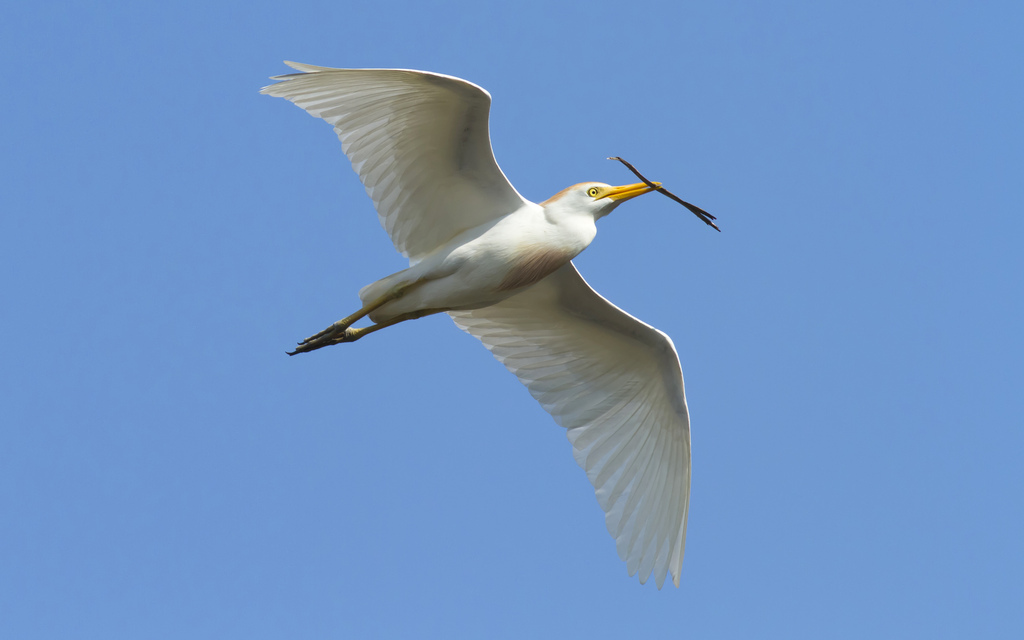
\includegraphics[width=1\linewidth]{./plots/cattle_egret.jpg}
  \begin{itemize} \setlength{\itemsep}{0.5em}
    \item eBird frequency: 2\%
    \item \alert{Photo credit}: Manjith Kainickara (Wikipedia)
  \end{itemize}

  \column{0.55\linewidth}
  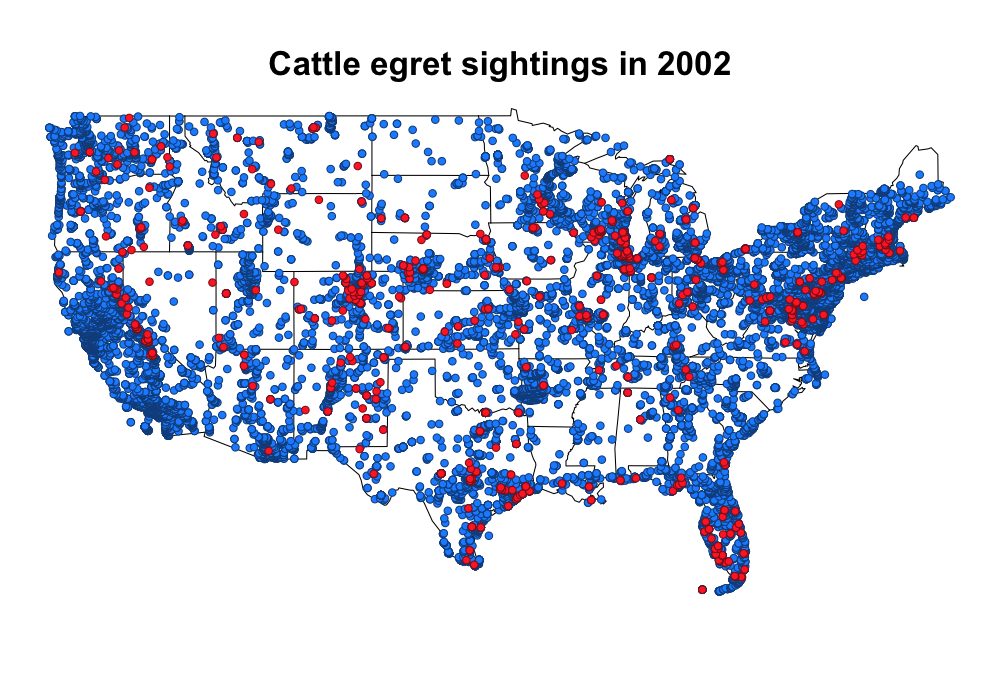
\includegraphics[width=1\linewidth]{./plots/cattle_egret.png}\\
  All reported sightings in 2002. \alert{Red} indicates a cattle egret sighting
\end{columns}
\end{frame}

\begin{frame}{Species 2: Vesper sparrow}
\begin{columns}[c]
  \column{0.45\linewidth}
  Vesper sparrow (Pooecetes gramineus): \vspace{0.5em}
  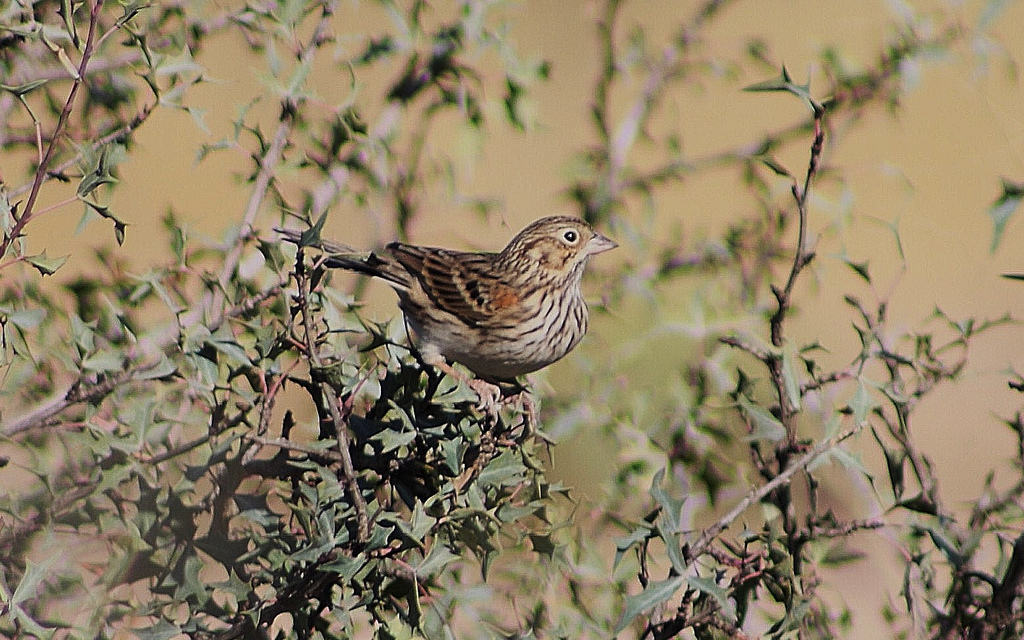
\includegraphics[width=1\linewidth]{./plots/vesper_sparrow.jpg}
  \begin{itemize} \setlength{\itemsep}{0.5em}
    \item eBird frequency: 1--2\%
    \item \alert{Photo credit}: Tripp Davenport (Flickr)
  \end{itemize}

  \column{0.55\linewidth}
  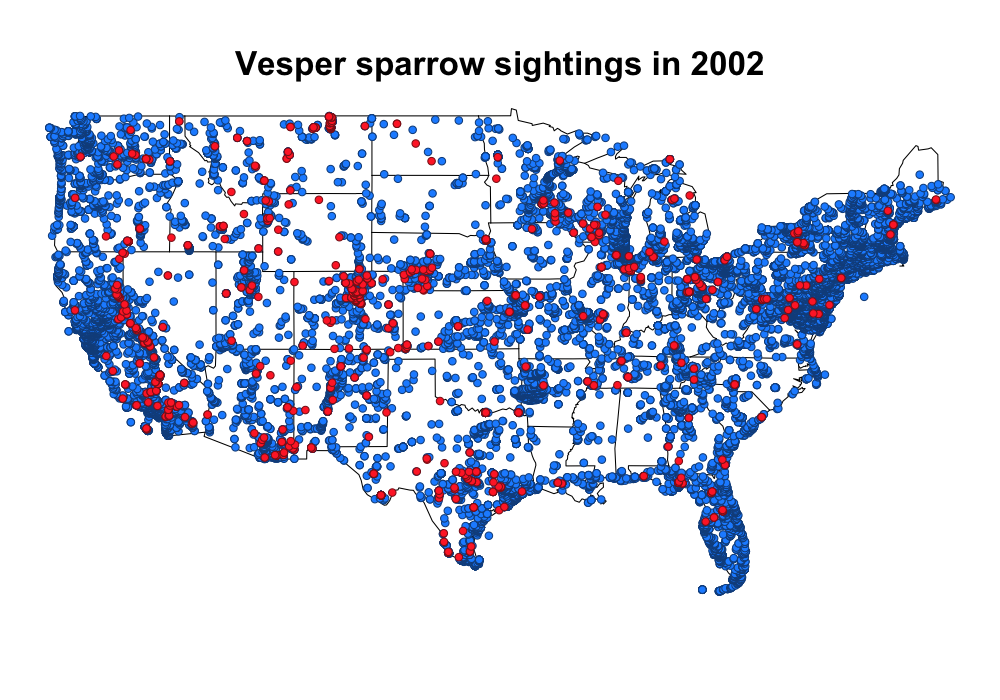
\includegraphics[width=1\linewidth]{./plots/vesper_sparrow.png}\\
  All reported sightings in 2002. \alert{Red} indicates a vesper sparrow sighting
\end{columns}
\end{frame}

\begin{frame}{Binary regression}
% logit, probit, cloglog
\begin{itemize} \setlength{\itemsep}{1em}
  \item Response is either 0 or 1
  \item Goal is to understand $P(Y_i = 1) = g(\bX_i \bbeta)$ where
  \begin{itemize} \setlength{\itemsep}{0.5em}
    \item $\bX_i$ is a $p$-vector of covariates for response $i$
    \item $\bbeta$ is a $p$-vector of regression parameters
    \item $g(\cdot) : \calR \rightarrow (0, 1)$
  \end{itemize}
\end{itemize}
\end{frame}

\begin{frame}{Binary regression}
\begin{itemize} \setlength{\itemsep}{1em}
  \item Common link functions:
  \begin{itemize} \setlength{\itemsep}{0.5em}
    \item Logit:
    \begin{align*}
      g(\bX_i \bbeta) = \frac{ \exp(\bX_i \bbeta) }{ 1 + \exp(\bX_i \bbeta) }
    \end{align*}
    \item Probit:
    \begin{align*}
      g(\bX_i \bbeta) = \Phi(\bX_i \bbeta)
    \end{align*}
    where $\Phi$ is the standard normal CDF
    \item Cloglog:
    \begin{align*}
      g(\bX_i \bbeta) = 1 - \exp[\exp(\bX_i \bbeta)]
    \end{align*}
  \end{itemize}
\end{itemize}
\end{frame}

\begin{frame}{Generalized extreme value (Wang and Dey, 2010)}
% cloglog is a special case of gev, Wang and Dey
\begin{itemize} \setlength{\itemsep}{1em}
  \item Link function is defined as
  \begin{align*}
    g(z_i) = 1 - \exp(-z_i)
  \end{align*}
  where
  \begin{align*}
    z_i = \left\{ \begin{array}{ll}
      (1 - \xi \bX_i \bbeta)^{-1 / \xi} & \xi \neq 0 \\[0.5em]
      \exp(-\bX_i \bbeta) & \xi = 0
      \end{array} \right.
  \end{align*}
  is standardized to give unit Fr\'{e}chet distribution.
  \item Note: The cloglog link is a special case when $\xi = 0$
\end{itemize}
\end{frame}

\begin{frame}{Spatial setting: Logit and probit}
\begin{itemize} \setlength{\itemsep}{1em}
  \item For logit and probit settings:
  \begin{itemize} \setlength{\itemsep}{0.5em}
    \item Assume an underlying Gaussian process for the latent variable
    \begin{align*}
      \bZ \sim \text{N}_n(\bX \bbeta, \bSigma)
    \end{align*}
    where
    \begin{itemize} \setlength{\itemsep}{0.25em}
      \item $\bX$ is an $n \times p$ matrix of covariates
      \item $\bbeta$ is defined as before
      \item $\bSigma$ is an $n \times n$ positive-definite covariance matrix
    \end{itemize}
    \item Conditional on $z(\bs_i)$
    \begin{align*}
      Y(\bs_i) \ind \text{Bern} \{g[z(\bs_i)]\}
    \end{align*}
  \end{itemize}
  \item \alert{Problem}: Asymptotic dependence for a multivariate Gaussian distribution is 0 unless correlation is 1.
\end{itemize}
\end{frame}

\begin{frame}{Spatial setting: GEV}
% when we assume the latent variable comes from a GEV, we should use a
% max-stable process
\begin{itemize} \setlength{\itemsep}{1em}
  \item If we believe the underlying distribution is extremal, then the dependence structure should match
  \item Multivariate GEV distributions are more challenging to work with than multivariate Gaussian distributions
  \item Interested in the \alert{asymptotic dependence} (i.e. dependence in the tail of the distribution):
  \begin{itemize} \setlength{\itemsep}{0.5em}
    \item Extremal index: Effective number of independent replications
    \item $\chi$-statistic:
    \begin{align*}
      \chi = \lim_{c \rightarrow c^*} P[Y(\bs_2) > c \mid Y(\bs_1) > c]
    \end{align*}
    where $c^*$ is the upper limit of the support of $Y$
  \end{itemize}
\end{itemize}
\end{frame}

\begin{frame}{Max-stable processes}
\begin{itemize} \setlength{\itemsep}{1em}
  \item Max-stable process is the extremal analogue to the Gaussian process
  \item Dependence structures are very flexible, but can be very challenging to work with in high dimensions
  \begin{itemize} \setlength{\itemsep}{0.5em}
    \item Pairwise composite likelihood (Padoan et al., 2010)
    \item Recent work allows for higher dimensions (Engelke et. al, 2014; Wadsworth and Tawn, 2014)
  \end{itemize}
\end{itemize}
\end{frame}

\begin{frame}{Dimension reduction}
% to help with large datasets, we use a random effects representation
% get dimension reduction with a grid of knots
\begin{itemize} \setlength{\itemsep}{1em}
  \item \alert{Problem}: For very large $n$ computational challenges arise
  \item Consider a set of $L << n$ knots $\bv_1, \ldots, \bv_L$
  \item We assume that the latent variables at the $n$ locations can be represented by a function of $L$ random effects
  \begin{itemize} \setlength{\itemsep}{0.5em}
    \item Logit and probit methods use Gaussian predictive process
    \item For the GEV, we propose using the hierarchical model for extremes by Reich and Shaby (2012)
  \end{itemize}
\end{itemize}
\end{frame}

\begin{frame}{Random effects representation}
  \begin{itemize} \setlength{\itemsep}{1em}
    \item Logit and probit use a Gaussian predictive process
    \begin{align*}
      \left[ \begin{array}{c}
        \bz_n \\
        \bz_L
      \end{array} \right]
      \sim \text{N}_{n + L} \left(
      \left[ \begin{array}{c}
        \bX_n \\
        \bX_L
      \end{array} \right] \bbeta,
      \left[ \begin{array}{cc}
        \Sigma_{nn} & \Sigma_{nL} \\
        \Sigma_{Ln} & \Sigma_{LL}
      \end{array} \right]
      \right)
    \end{align*}
    \item We fit the model using the latent variables at the knot locations
    \item Use distribution of $\bz_n | \bz_L$ to get back distribution at all sites
  \end{itemize}
\end{frame}

\begin{frame}{Max-stable processes: A hierarchical representation (Reich \& Shaby, 2012)}
\begin{itemize} \setlength{\itemsep}{1em}
  \item Let $\widetilde{\bY} \sim \text{GEV}_n[\mu(\bs), \sigma(\bs), \xi(\bs)]$ be a realization from multivariate generalized extreme value distribution
  \item Consider a set of $L$ knots, $\bv_1, \ldots, \bv_L$
  \item Model the spatial dependence using
  \begin{align*}
    \footnotesize
    \theta(\bs) = \left[\sum_{l = 1}^L A_l w_l(\bs)^{1 / \alpha}\right]^\alpha
  \end{align*}
  where
  \begin{itemize} \setlength{\itemsep}{0.5em}
    \item $A_l$ are i.i.d. positive stable random effects
    \item $w_l(\bs)$ are a set of non-negative scaled kernel basis functions, scaled so that $\sum_{l = 1}^L w_l(\bs) = 1$
    \item $\alpha \in (0, 1)$ is a parameter controlling strength of spatial dependence (0: high, 1: independent)
  \end{itemize}
  % \item We follow Reich and Shaby (2012) and use Gaussian weights
  % { \footnotesize
  %   \begin{align*}
  %     w_l(\bs_i) = \frac{ \exp\left[ -0.5 \left( \frac{ || \bs_i - \bv_l || }{ \rho} \right)^2 \right]}{ \sum_{l = 1}^L \exp\left[ -0.5 \left( \frac{ || \bs_i - \bv_l || }{ \rho} \right)^2 \right] }
  %   \end{align*}
  % }
\end{itemize}
\end{frame}

\begin{frame}{Max-stable processes: A hierarchical representation (Reich \& Shaby, 2012)}
\begin{itemize} \setlength{\itemsep}{1em}
  \item When conditioning on $\theta$
  \begin{align*}
    \widetilde{Y}(\bs_i) \mid A_l &\ind \text{GEV}[\mu^*(\bs_i), \sigma^*(\bs_i), \xi^*(\bs_i)] \\
    A_l &\iid \text{PS}(\alpha)
  \end{align*}
  where
  \begin{itemize} \setlength{\itemsep}{0.5em}
    \item $\mu^*(\bs_i) = \mu(\bs) + \frac{\sigma(\bs)}{\xi(\bs)}[\theta(\bs)^{\xi(\bs)} - 1]$
    \item $\sigma^*(\bs_i) = \alpha \sigma(\bs) \theta(\bs)^{\xi(\bs)}$
    \item $\xi^*(\bs) = \alpha \xi(\bs)$
  \end{itemize}
\end{itemize}
\end{frame}

\begin{frame}{Proposed Method}
  \begin{itemize} \setlength{\itemsep}{1em}
    \item Fit a hierarchical random effects model using MCMC
    \begin{itemize} \setlength{\itemsep}{0.5em}
      \item Extends model from Reich and Shaby (2012)
      \item Using random walk Metropolis-Hastings algorithm
      \item Pairwise composite likelihood estimates used for initial values and hyperparameters in MCMC
    \end{itemize}
  \end{itemize}
\end{frame}

% \begin{frame}{Pairwise composite likelihood}
%   \begin{itemize}
%     \item We use a censored pairwise composite likelihood
%     \begin{itemize}
%       \item Marginalizes out random effects
%     \end{itemize}
%     \item Common in extremes
%     \begin{itemize}
%       \item Bivariate distributions are computationally tractible
%       \item Only latent values where $Y = 1$ inform likelihood
%     \end{itemize}
%   \end{itemize}
% \end{frame}

\begin{frame}{Hierarchical MCMC}
  \begin{itemize} \setlength{\itemsep}{1em}
    \item Data:
    \begin{align*}
      Y(\bs_i) | g[z(\bs_i)] \ind \text{Bern}\{g[z(\bs_i)]\}
    \end{align*}
    \item Latent process:
    \begin{align*}
      g[z(\bs_i)] &= 1 - \exp\left\{ \sum_{l = 1}^L A_l \left[\frac{ w_l (\bs_i) }{z_i} \right]^{1 / \alpha} \right\}\\
    \end{align*} \vspace{-0.5em}
    where
    \begin{align*}
      z_i &= \left\{ \begin{array}{ll}
        (1 - \xi \bX_i \bbeta)^{-1 / \xi} & \xi \neq 0 \\
        \exp(-\bX_i \bbeta) & \xi = 0
        \end{array} \right.\\
      A_l &\iid \text{PS}(\alpha)
    \end{align*}
  \end{itemize}
\end{frame}

\begin{frame}{Simulation study: Settings}
  \begin{itemize} \setlength{\itemsep}{0.5em}
    \item Conducting a simulation study with 50 datasets generated from our model with strong spatial dependence with knots on a $31 \times 31$ grid
    \item Looking at impact of number of observations as well as prevalence
  \end{itemize}
  \centering
  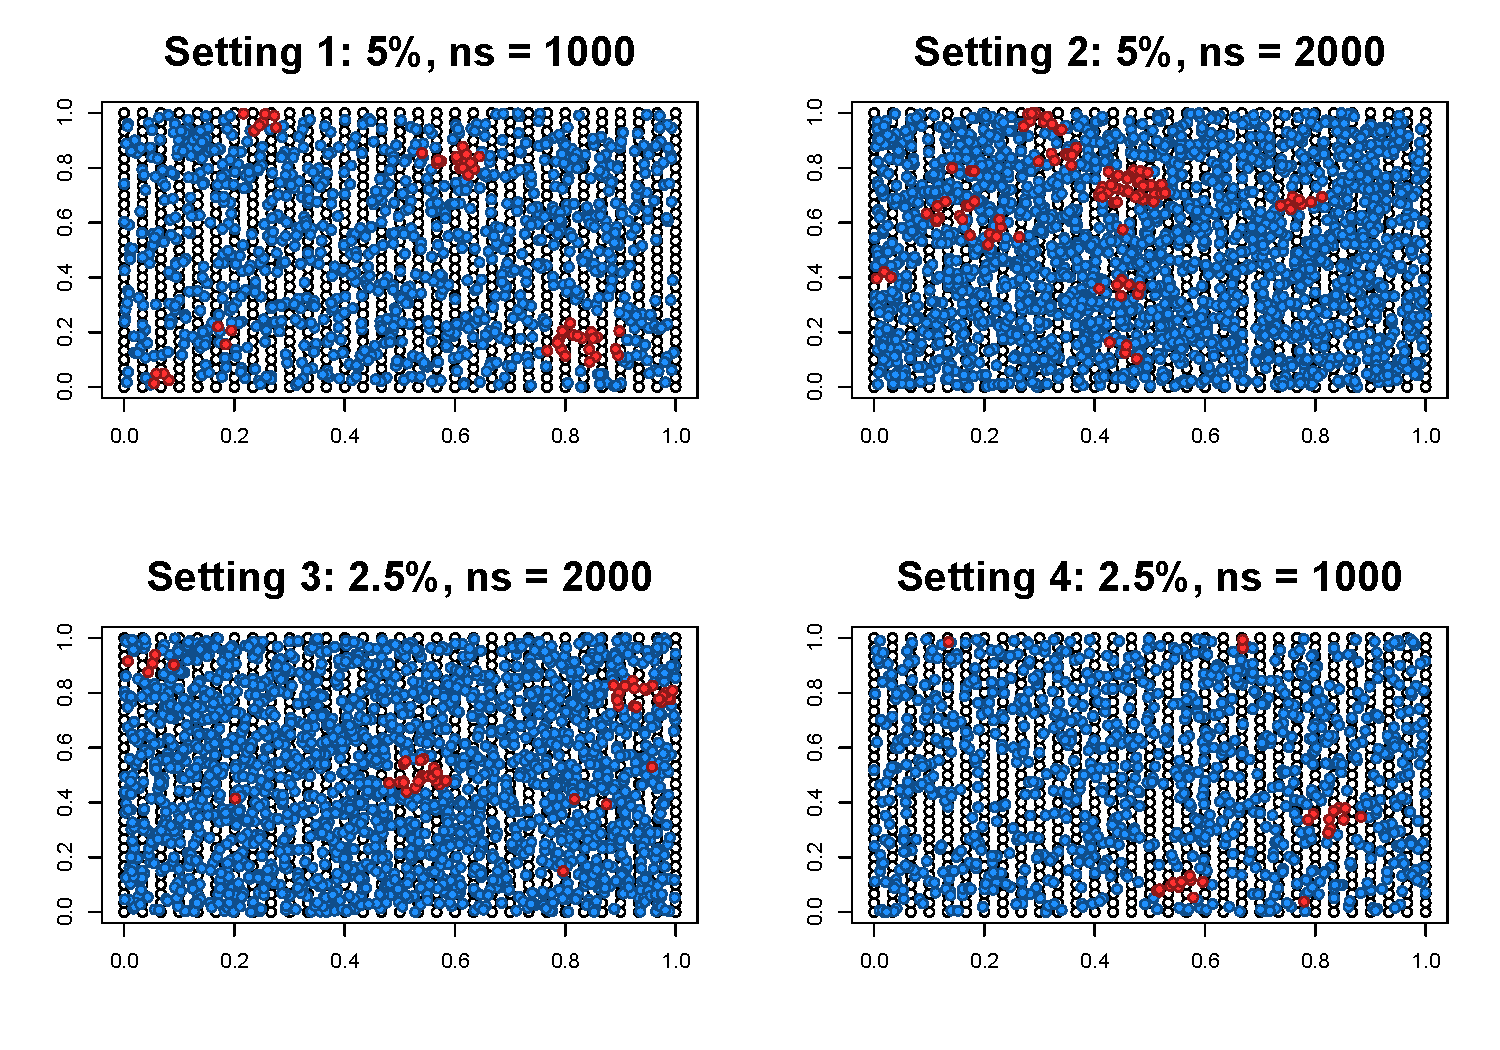
\includegraphics[width=0.7\linewidth]{./plots/simulated_data.pdf}
\end{frame}

\begin{frame}{Simulation study: Methods}
  \begin{itemize} \setlength{\itemsep}{1em}
    \item Fitting Bayesian models for spatial probit, spatial logit ({\tt spBayes::spGLM}) and spatial GEV (fixing $\xi = 0$ for identifiability)
    \item Model fit using 75\% of the observations as a training set and 25\% for cross-validation
    \item Measuring performance with the Brier score (Gneiting and Raftery, 2007)
  \end{itemize}
\end{frame}

\begin{frame}{Simulation study: Preliminary results and future work}
  \begin{itemize} \setlength{\itemsep}{1em}
    \item Preliminary results:
    \begin{itemize} \setlength{\itemsep}{0.5em}
      \item Our model demonstrates some improvement over the spatial probit model (75\%--85\% reduction in Brier score)
      \item Using adaptive MCMC with {\tt spBayes::spGLM} is very slow with this many knots, and still waiting on results (on order of 5--6 times longer on a single-threaded BLAS)
    \end{itemize}
    \item Future work:
    \begin{itemize} \setlength{\itemsep}{0.5em}
      \item Cluster size and smoothness of the field impacts which methods do better
      \item Exploring impact of reducing number of knots
      \item Data analysis with eBirds data
    \end{itemize}
  \end{itemize}
\end{frame}

\begin{frame}{Questions}
  \begin{itemize} \setlength{\itemsep}{1em}
    \item Questions?
    \item Thank you for your attention.
  \end{itemize}
\end{frame}

\begin{frame}[allowframebreaks]{References}
  \footnotesize
  \begin{itemize} \setlength{\itemsep}{1em}
    \item Coles, S., Heffernan, J. and Tawn, J. (1999) Dependence Measures for Extreme Value Analyses. \emph{Extremes}, \textbf{2}, 339--365.
    \item Engelke, S., Malinowski, A., Kabluchko, Z. and Schlather, M. (2014) Estimation of H\"{u}sler-Reiss distributions and Brown-Resnick processes. \emph{Journal of the Royal Statistical Society. Series B: Statistical Methodology}, \textbf{77}, 239--265.
    \item Padoan, S. A., Ribatet, M. and Sisson, S. A. (2010) Likelihood-Based Inference for Max-Stable Processes. \emph{Journal of the American Statistical Association}, \textbf{105}, 263--277.
    \item Reich, B. J. and Shaby, B. A. (2012) A hierarchical max-stable spatial model for extreme precipitation. \emph{The Annals of Applied Statistics}, \textbf{6}, 1430--1451.
    \item Sullivan, B. L., Wood, C. L., Iliff, M. J., Bonney, R. E., Fink, D. and Kelling, S. (2009) eBird: A citizen- based bird observation network in the biological sciences. \emph{Biological Conservation}, \textbf{142}, 2282--2292.
    \item Wadsworth, J. L. and Tawn, J. a. (2014) Efficient inference for spatial extreme value processes associated to log-Gaussian random func- tions. \emph{Biometrika}, \textbf{101}, 1--15.
    \item Wang, X. and Dey, D. K. (2010) Generalized extreme value regression for binary response data: An ap- plication to B2B electronic payments system adoption. \emph{The Annals of Applied Statistics}, \textbf{4}, 2000--2023.
  \end{itemize}
\end{frame}

\end{document}